\documentclass[12pt]{article}
% Эта строка — комментарий, она не будет показана в выходном файле
\usepackage{ucs}
\usepackage[utf8x]{inputenc} % Включаем поддержку UTF8
\usepackage[russian]{babel}  % Включаем пакет для поддержки русского языка
\usepackage{amsmath}
\usepackage{amssymb}
\usepackage{mathtools}
\usepackage{graphicx}
\graphicspath{ {/Users/sergmiller/Documents/tex/formal/dfa1/} }

\title{Домашнее задание № 2}
\date{\today}
\author{Сергей Миллер 494}

\begin{document}
 	\maketitle
	\textbf{Задача 1.}
 	
  	\textbf{a)}
      Построим автомат прямо по регулярному выражению(вершина серого цвета - начальная, вершины в виде двойного круга - конечные):

      %\includegraphics[width=0.5\linewidth]
      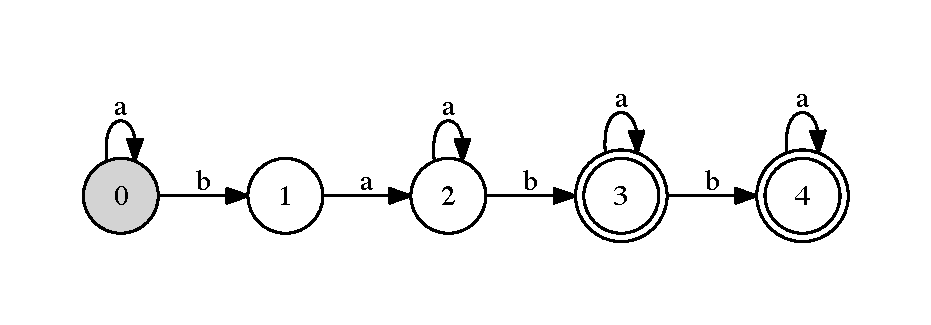
\includegraphics{state_machine1.pdf}
    
    \begin{equation}
      a^{*}ba^{+}ba^{*}(ba^{*} + 1)
    \end{equation}
    Очевидно,что он является ДКА. (Видимо причина $\textit{интуитивного}$ построения этого ДКА в том, что данное регулярное выражение задает однозначный разбор слова на блоки)
 	
    \textbf{б)}
      Сначала построим НКА(с однобуквенными и возможно $\varepsilon$ переходами):

      \begin{figure}  
      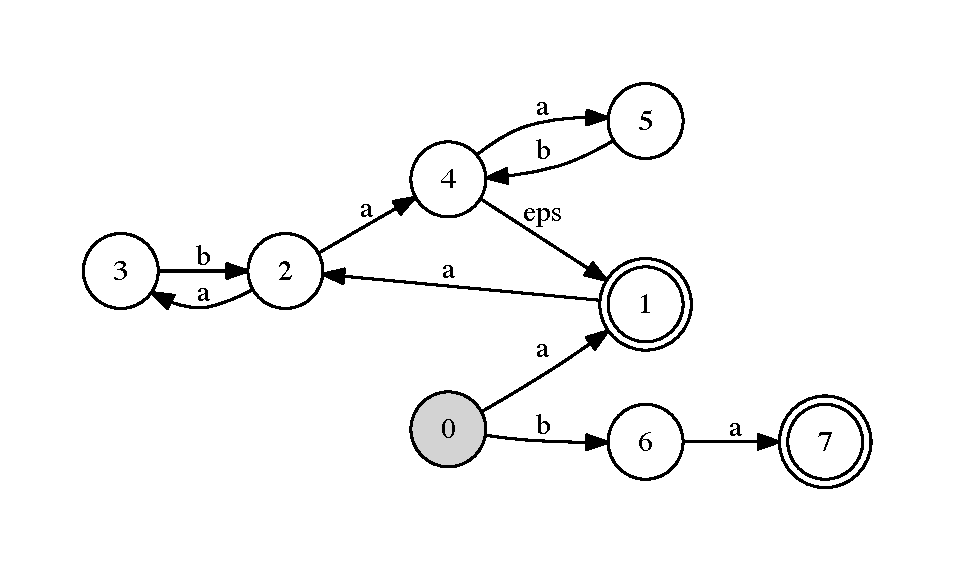
\includegraphics{state_machine2.pdf}
      % После избавимся от единственного $\varepsilon$ перехода:
       \text{После избавимся от единственного $\varepsilon$ перехода:}
      \end{figure}

      \begin{equation}
      a(a(ab)^{*}a(ab)^{*})^{*} + ba
    \end{equation}

    
   
      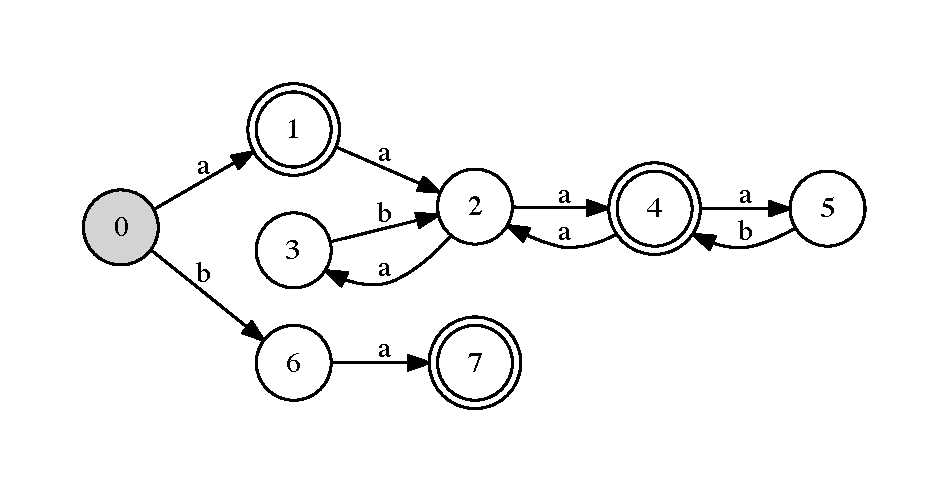
\includegraphics{state_machine2_1.pdf}
      \text{Теперь по известному алгоритму построим ДКА для данного автомата:} 

   
   %Теперь по известному алгоритму построим ДКА для данного автомата:

    \begin{array}{c|c|c}
      

      0 & a & 1 \\
      0 & b & 6 \\
      \hline
      1 & a & 2 \\
      \hline
      6 & a & 7 \\
      \hline
      2 & a & 3,4 \\
      \hline
      3,4 & a & 2,5 \\
      3,4 & b & 2 \\
      \hline
      2,5 & a & 3,4 \\
      2,5 & b & 4 \\
      \hline
      4 & a & 2,5 \\

    \end{array}

  \maketitle
    \text{Ответ:}
      
      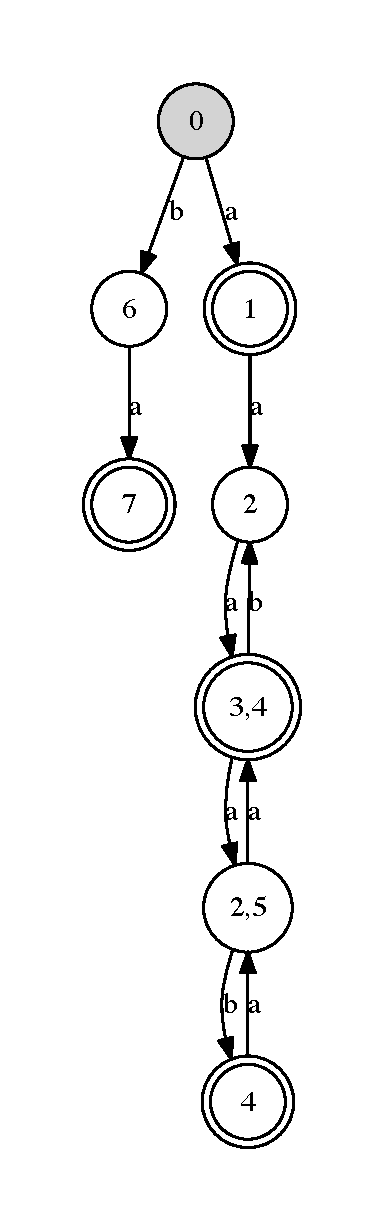
\includegraphics{state_machine2_2.pdf}

  \maketitle
    \textbf{Задача 2.}
      Рассмотрим $L = L(a + 1)$ и какой нибудь НКА $M =  M(L)$, имеющий только с однобуквенные переходы и ровно одно завершающе состояние. Так как язык содержит пустое слово, то $q_0 \in F$. Теперь рассмотрим путь в этом автомате, по которому распознается $a$. Пусть в автомате  $\Delta \supset \langle q_0, a \rangle \mapsto q_0 $. Но тогда $L \supset L^{'} = a^{*}$. Иначе рассмотрим второй случай: $ \exists q \neq q_0 \in Q : \langle q_0, s \rangle \mapsto q \ , s \in \Sigma$.(В слуачае отсутствия и этого ребра $L = 1$). Но тогда для распознования $a$ должен существовать путь из $q_0$ в $q_0$ длины 1, чего очевидно не может быть при однобуквенных переходах и отсутствии $\langle q_0, a \rangle \mapsto q_0 $. 

    \textbf{Задача 3.}
      Ответ: неверно.

      Рассмотрим язык $L: \varepsilon \notin L$. Построим  произвольный НКА $M = M(L)$. Теперь рассмотрим его завершающие состояния. Очевидно, что $q_0 \notin F$. Тогда проведем следующую процедуру: для каждой конечной вершины $q_f \in M$ создадим копию $q^{'}_f$ c теми же входящими ребрами что и у $q_f$, кроме ребер вида $\langle q_f, s \rangle \mapsto q_f$. А все $q^{'}_f$ объединим в одну конечную вершину $q_F$. Также добавим связей: $(\langle q_f, s \rangle \mapsto q_F) \forall s: \exists \langle q_f, s \rangle \mapsto q_f$. (См. рис. после задач) Покажем, что полученный ДКА $M^{'}$ распознает тот же язык. Пусть $w \in L$. Тогда в $M$ найдется путь из $q_0$ в какой-то $q_f$. То есть $w = ab, b \in \Sigma, \exists q: \langle q_0, ab \rangle \mapsto \langle q, b \rangle \mapsto \langle q_f, \varepsilon \rangle$. Но тогда в обоих случаях: $q = q_f$ или $q \neq q_f$ получаем $M^{'}: \langle q_0, ab \rangle \mapsto \langle q, b \rangle \mapsto \langle q_F, \varepsilon \rangle$ по построению $M^{'}$. Следовательно $L(M) \subset L(M^{'})$. Обратно: пусть $w \in L(M^{'})$. Рассмотрим вершину $q$ перед $q_F$ на пути в $M^{'}$, который реализует слово $w$. Если $q$ это не копия одной из вершин $q_f \in M$, то в $M$ существует такой же путь  $\Rightarrow w \in M$. Иначе, $(\exists \langle q, s \rangle \mapsto q) \forall s: \langle q, s \rangle \mapsto q_F$ по построению $M^{'}$.  Значит $w = as: s \in \Sigma$ и в $M$ слово $w$ реализуется следующим образом: $\langle q_0, as \rangle \mapsto \langle q_f, s \rangle \mapsto \langle q_f, \varepsilon \rangle$. 
      \begin{figure}[H]
      \text{Поясняющий рисунок к 3 задаче}
      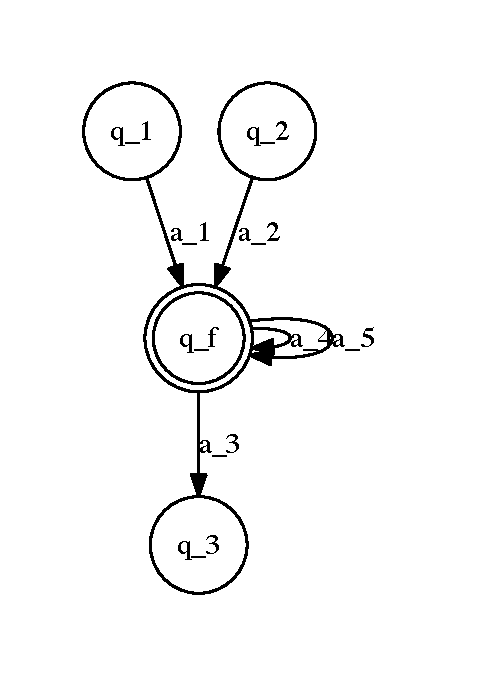
\includegraphics{state_machine2_3.pdf}
      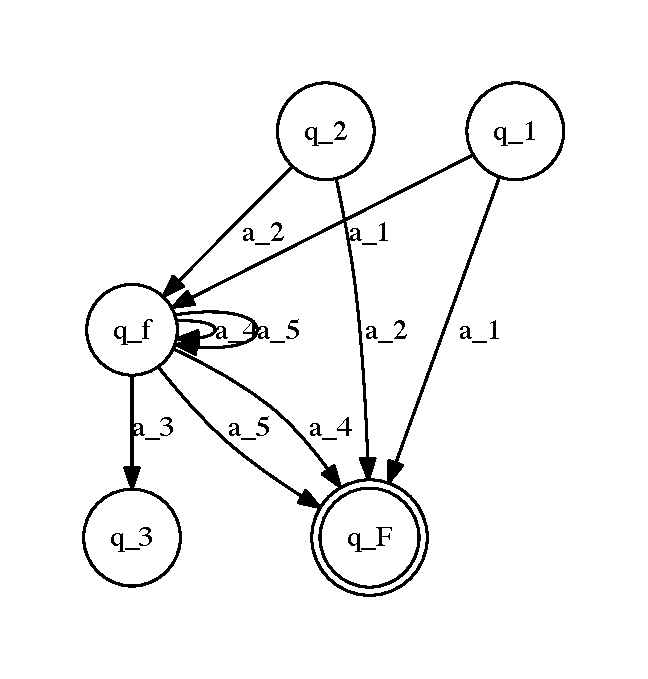
\includegraphics{state_machine2_4.pdf}
      \end{figure}

    \textbf{Задача 4.}
       Ответ: можно.

       Построим произвольный НКА $M = M(L)$. Очевидно, что если $\varepsilon \in L$, то $q_0 \in F$(Так как все переходы однобуквенные). Воспользуемся процедурой построения автомата $M^{;}$ из предыдущей задачи $\forall q_f \in F: q_f \neq q_0$. В точности тем же методом можно доказать, что $L(M) = L(M^{'})$. При этом количество конечных состояний у $M^{'}$ ровно 2. Для языков, не содержащих $\varepsilon$, воспользуемся решением предыдущей задачи и обойдемся одним выходом.

\end{document}